%%%%%%%%%%%%%%%%%%%%%%%%%%%%%%%%%%%%%%%%%%%%%%%%%%%%%%%%%%%%%%%%%%%%%%%%%%%%%%%
%% About this LaTeX file:
%%
%% This is a sample LaTeX file for a UWaterloo exam/test document using the 
%% Odyssey exam management system and the Crowdmark online grading system.
%% Both Odyssey and Crowdmark cover over parts of every test page.
%% This LaTeX file sets up a page layout with this in mind.

%% Look for this LaTeX file on the University of Waterloo's
%% help page for the Crowdmark system: https://uwaterloo.ca/crowdmark/
%% or https://uwaterloo.ca/crowdmark/midterms-and-final-exams.
%% Sample pdf files showing the page layout options are there too, as are
%% documents describing how to use the Odyssey and Crowdmark systems for
%% managing and grading (online grading) your tests, quizzes, and exams.

%% Why the page layout is the way it is:
%%
%% Odyssey uses the bottom .65 inches of every page for a page number
%% and about 4 inches at the top of the cover page for exam information.
%% Crowdmark uses the top 1.5 inches of every page (including the cover page)
%% for QR coded booklet/page information.
%% When Odyssey and Crowdmark are used together, the cover page starts
%% with a 1.5 inch QR code area followed by the Odyssey 4 inch exam area.

%% In fact, Odyssey can use as little as 3.75 inches when there are no special
%% materials listed for an exam.  And, it can use more than 4 inches when there
%% are many listed materials.

%% How to use this LaTeX file:
%%
%% This sample LaTeX file can be used for 4 variations of page layout.
%% Two variations are for Crowdmark, when the LaTeX variable tmargin is 
%% set to 1.5in (default):
%%   * Odyssey and Crowdmark: use the file as is
%%     (the cover page framed box with exam info is covered up by Odyssey)
%%   * Crowdmark without Odyssey: use the file as is 
%%     (the framed box is not covered up)
%%
%% And two variations that do not use Crowdmark, when the LaTeX 
%% variable tmargin is set to .25in (the larger Crowdmark top margin 
%% of 1.5 inches is no longer needed):
%%   * Odyssey without Crowdmark
%%   * Without Odyssey or Crowdmark

% Version 1 (Feb 19, 2019), Paul Kates (pkates@uwaterloo.ca).
%%%%%%%%%%%%%%%%%%%%%%%%%%%%%%%%%%%%%%%%%%%%%%%%%%%%%%%%%%%%%%%%%%%%%%%%%%%%%%%

\documentclass[12pt]{article}

\usepackage[utf8]{inputenc}
% Use showframe to see layout boundaries during drafts, but not for a printed
% exam.
%\usepackage{showframe}

%% Page layout
\usepackage{geometry}  % used for page layout
  % Size numbers you can change:
  % hmargin{leftside,rightside} page margins can be adjusted to your liking.
  % The page looks symmetric with the left, right values of .5in and .68in.
  %
  % Size numbers not meant for change.  Sizes are determined by the heights of
  % the areas covered by Odyssey and Crowdmark.
  % tmargin = margin along the top of every page 
  %         = 1.5 inches when used with Crowdmark, or
  %         = .25 inches when used without Crowdmark
  % bmargin = margin along the bottom of every page = .65 inches; from Odyssey
  % \myodysseyheight = height of this file's cover page exam info area
  %                    which is meant to fit inside (be covered up by)
  %                    the Odyssey exam info area (of about 4in in height
  \newlength{\myodysseyheight} 
  \setlength{\myodysseyheight}{3.6in}  % typical range [3.6,4] inches

  \geometry{letterpaper, % 8.5 x 11 inch page (legalpaper 8.5x14in also works)
          tmargin=1.5in, % page top margin when using Crowdmark
         %tmargin=.25in, % page top margin when not using Crowdmark
          hmargin={.5in,.68in}, % leftside, rightside page margins 
                                % (page looks symmetric)
          bmargin=.65in, % page bottom margin
          includehead    % place header in body of text below Crowdmark QR
          }

%% Footer and header
% The footer below will be covered up by Odyssey's footer.  But, when not using
% Odyssey, the footer will show the same information as Odyssey: exam title and
% page number.
\usepackage{lastpage}  % for page number of last page
\usepackage{fancyhdr}  % for setting footer
  \pagestyle{fancy}
  \fancyhead{}         % turn off default header and footer 
  \fancyfoot{}
  \fancyfoot[L]{University of Waterloo}  % left, centre, right footers
  \fancyfoot[C]{SE 465 Final Winter 2019}
  \fancyfoot[R]{Page \thepage\ of \pageref{LastPage}}

  \renewcommand{\headrulewidth}{0pt}     % really turn off header rule
  \renewcommand{\footrulewidth}{0.4pt}   % default is 0pt

%% Other LaTeX packages and settings you use can go here:
%
  \usepackage{mathtools, amssymb} % mathtools includes amsmath package
  \usepackage{enumitem}
  \usepackage{listings}
  \usepackage{url}
  \usepackage[T1]{fontenc}
  \usepackage[scaled]{beramono}
  \usepackage{XCharter}
  \lstset{basicstyle=\footnotesize\ttfamily,breaklines=true}

%% Question grade point values in left margin
\reversemarginpar  % put margin note/grade on left, default is rightside of page
\setlength{\marginparsep}{-.4in}  % default 10pt

%%%%%%%%%%%%%%%%%%%%%%%%%%%%%%%%%%%%%%%%%%%%%%%%%%%%%%%%%%%%%%%%%%%%%%%%%%%%%%%
%% Cover page of test:

\begin{document}
% Save original paragraph indentation size in case you want to restore it.
\newlength{\myoldparindent}
\setlength{\myoldparindent}{\parindent}
\setlength{\parindent}{0em}  % turn off paragraph indentation (set length to 0)
% Use following line later if ever want to restore \parindent:
%\setlength{\parindent}{\myoldparindent} 
 
% A framed box is placed around the area where Odyssey puts its cover page info.
% Anything put into this box will be covered up by Odyssey.
% You can put your exam info here for drafts.
% Or, use this area for your exam cover page if you decide not to use Odyssey.
% If you find that the box frame peeks below the Odyssey cover page info then
% either remove the framing lines by changing \fbox to \mbox below, or make 
% a small reduction in the size of value \myodysseyheight (set above).

\fbox{  % to remove the frame lines, change this \fbox to \mbox
% Start of a minipage container (inside the fbox) for 2 inner minipages below.
\begin{minipage}[t][\myodysseyheight]{\textwidth} 

% Some layout comments you can print on a draft cover page.
\begin{center}
%\large{\textbf{Space above this box is for a Crowdmark QR code}}\\[1ex]
%\large{\textbf{This boxed area will be covered up by Odyssey}}\\[2ex]

% Exam title information.
%
SE 465 Final Examination\\
University of Waterloo\\
Term: Winter \hspace{1cm} Year: 2019\\
\end{center}
% Required UWaterloo exam details for cover page:
\begin{minipage}[t]{3.5in} % half of the default 7 in page text width
Date: Tuesday, April 23, 2019\\
Time: 12:30 – 15:00 (150 minutes)\\
Instructors: Patrick Lam\\
Lecture Section: 001\\
Exam Type: Open book, open notes, calculators with no communications capabilities\\
Number of non-blank exam pages (includes cover page): 13\\
\end{minipage}  % end of first inner minipage of cover page exam details
\hfill%
%
% Student information area:
\begin{minipage}[t]{3.5in} % half of the page text width
\textit{Please Print}\\[1mm]
Last Name \hrulefill\\[2mm]
First Name \hrulefill\\[2mm]
UWaterloo ID \# \hrulefill\\[2mm]
Username \hrulefill\\[2mm]
\end{minipage} % end of second inner minipage of cover page student details
\end{minipage} % end of framed box container minipage
}

%% "Instructions to students" area of the cover page.
%% Every item here is optional.  Even the grading box is here only as 
%% an example.
%
% Adjust the vertical space here if the Odyssey exam info area grows larger
% and starts to cover up the grading box below.
%\vspace{1in}   % height can be 0 to 1 inch to nicely position the grading box
% Grading box.  Use the "Score" row for student scores if not using Crowdmark.
\begin{center}
 \begin{tabular}{|l| c c c c c c c ||r|} \hline
 Question & 1 & 2.1 & 2.2 & 3 & 4 & 5 & 6 &Total \\ \hline
 Points & 30 & 10 & 10 & 20 & 20 & 20 & 10 & 120 \\ \hline
 %Score  &    &    &    &    &    &    &    &    &    &    &    \\ \hline
 \end{tabular}
\end{center}
%
\textbf{Instructions}
\begin{enumerate}
   \item Turn off all communication devices. Communication devices must be stored with your personal items for the duration of the exam. Taking a communication device to a washroom break during this examination is not allowed and will be considered an academic offence.
    \item I shuffled the order of the questions from what I said in class for better page breaks.
    \item The exam lasts \textbf{150} minutes and there are 120 marks.
    \item Verify that your name and student ID number is on the cover page.
    \item If you feel like you need to ask a question, know that the most likely answer is ``Read the Question''. No questions are permitted. If you find that a question requires clarification, proceed by clearly stating any reasonable assumptions necessary to complete the question. If your assumptions are reasonable, they will be taken into account during grading. 
\item Answer the questions in the spaces provided.  If you require 
additional space to answer a question, please use the second last page 
and refer to this page in your solutions. You may tear off the last page 
to use for rough work.
\item Do not write on the Crowdmark QR code at the top of each page.
\item Use a dark pencil or pen for your work.
% \item More instructions, about calculators, formula sheets, asking 
% questions, etc.
\end{enumerate}

% Remove these 2 LaTeX commands when making your own cover page.

%%%%%%%%%%%%%%%%%%%%%%%%%%%%%%%%%%%%%%%%%%%%%%%%%%%%%%%%%%%%%%%%%%%%%%%%%%%%%%%
%% Second page of test, for exam questions.
%
\newpage
\renewcommand{\headrulewidth}{0.4pt}  % put header rule on all non-cover pages 



\section{Short Answer [30 marks total]}
Answer these questions using at most three sentences. Each question is worth 3 points.

\begin{enumerate}[label=(\alph*)]
%\paragraph{Fuzzing}
\item In class, we discussed hierarchical fuzzing for compilers and web browsers. Give one
example of software, or a software component, besides compilers and web browsers,
where you could use hierarchical fuzzing.
\vspace*{8em}

%\paragraph{Bug-finding Tools: Static}
\item Name a static bug-finding tool and give an example of a
false positive that this tool is subject to.
\vspace*{8em}

%\paragraph{Bug-finding Tools: Dynamic}
\item
Name a dynamic bug-finding tool and explain a case where this tool
will miss an error that the tool was built to find.
\vspace*{8em}

%\paragraph{Continuous Integration}
\item Assume that every developer always runs all existing tests on their
local system before pushing their changes. Describe a class of code
issue that Continuous Integration can still catch even in this ideal
situation.
\vspace*{8em}

%\paragraph{Parts of a Test}
\item Classify each of the lines of the following test as one of: setup
(S)/teardown (T)/exercising system (E)/verifying results
(V).

\begin{lstlisting}
     @Test
     public void testAlternateMarker() throws Throwable {
         PMD p = new PMD();
         p.getConfiguration().setSuppressMarker("FOOBAR");
         RuleContext ctx = new RuleContext();
         Report r = new Report();
         ctx.setReport(r);
         ctx.setSourceCodeFilename("n/a");
         ctx.setLanguageVersion(LanguageRegistry.getLanguage(JavaLanguageModule.NAME).getDefaultVersion());
         RuleSet rules = new RuleSet();
         rules.addRule(rule);
         p.getSourceCodeProcessor().processSourceCode
             (new StringReader(TEST3), new RuleSets(rules), ctx);
         assertTrue(r.isEmpty());
         assertEquals(r.getSuppressedRuleViolations().size(), 1);
     }
\end{lstlisting}

%\paragraph{State vs. Behaviour}
\item Does test {\tt testAlternateMarker()} above verify state or behaviour? Explain why.
\vspace*{8em}
  
%\paragraph{Code Review}
\item Write down one advantage and one disadvantage of having your code reviewed, in terms of producing better software.

\newpage
%\paragraph{Summarizing a Bug Report}
\item Propose a one-line summary for the following Mozilla Firefox bug report (\#1513270).

\begin{quote}
\emph{Steps to reproduce:}

Opening the attached imgbug.html file shows 2 paragraphs, each with an image.

\emph{Actual results:}

The Orca screen reader only sees the second image, because the first one is exposed through AT-SPI with the `invalid' state attribute, which Orca uses to filter out buggy or dysfunctional objects.  This is quite legitimate on Orca's part, as this state should not be present in a properly behaving object.

I have no idea yet why Firefox adds the `invalid` attribute on the first image yet not on the second, the only difference is the image data which renders fine in both cases, and seem legitimate to me.  The first comes from the original site problem (dragonium.net), and the second is a Gimp-saved version of the first.

\emph{Expected results:}

Both images should be recognized and vocalized by the Orca screen
reader. Image data shouldn't affect this, as the alt and/or title
attributes are used, and present in both cases.  The AT-SPI object
shouldn't expose the `invalid` state.

Tested with FF52 and 60, but likely to affect all versions.
\end{quote}

\vspace*{8em}

%\paragraph{MUST-beliefs}
\item What can you deduce about {\tt n} if the second statement below successfully executes?
\begin{lstlisting}[numbers=left]
  struct node * n = calloc(1, sizeof(struct node));
  n->data = 5;
\end{lstlisting}
\vspace*{8em}

\newpage
%\paragraph{Round Trip Coverage}
\item You have a Finite State Machine describing your system and your test suite achieves Complete Round Trip Coverage.
This test suite could still miss important system behaviours. Explain how you would improve your test suite
while still keeping it FSM-based.
\vspace*{6em}
\end{enumerate}

\section{Not-so-short Answer [20 marks]}


\subsection{Nullable Types [10 marks]}
Consider the following code, which includes a {\tt @Nullable} annotation.
\begin{lstlisting}[numbers=left]
  void bar() {
    BufferedReader reader;
    try {
      reader = new BufferedReader(new FileReader("se465-final.txt"));
      readFile(reader);
    } catch (IOException e) {}
    reader.close();
  }

  void readFile(@Nullable BufferedReader r) {
    String s = r.readLine();
    if (s != null)
      System.out.println(s);
  }
\end{lstlisting}

(a) Which runtime exception can crash this code? (b) From what we see
here, is the {\tt @Nullable} annotation for {\tt readFile} necessary?
What modification would make it necessary? (c) Would {\tt readFile()}
pass FB Infer Eradicate as you see it here? How would you fix {\tt
  readFile()} to make it pass?

\vspace*{13em}

\subsection{Mutation [10 marks]}
Consider test suite $T$, original program $p$, and mutant $m$. $T$ achieves statement coverage
on $m$ but not on $p$. Demonstrate $T$, $p$, and $m$ for which this might happen;
describe the mutation converting $p$ to $m$. Does your $T$ kill $m$? Why or why not?
\vspace*{16em}

\newpage
\section{Edge Coverage [20 marks]}
Provide test requirements and an input set that achieves edge coverage on this method.

\begin{lstlisting}
  public void foo(String s) {
    if (s.length() == 6)
      System.out.println("six");
    for (int i = 0; i < s.length(); i++) {
      if (Character.isAlphabetic(s.charAt(i)))
        System.out.print("r");
      System.out.print(s.charAt(i));
    }
  }
\end{lstlisting}

\newpage
\section{Mock Objects [20 marks]}
You are given the following code that represents a one dimensional world with transportation, with distances measured as integer kilometers and prices measured as integers.

\begin{lstlisting}
interface Transport {
    Vehicle hailVehicle();
    int getPricePerKm();
    int getBasePrice();
}

interface Vehicle {
    Driver getDriver();
    void waitUntilArrivedAt(int location);
}

interface Driver {
    void setDestination(int location);
    void pay(int amount);
}

interface Wallet {
    Wallet(int initialAmount);

    void takeOut(int amount) throws YouAreBrokeException;
    int getAmount();
}

class Person {
    Person(int home, int currentLocation, Wallet wallet) { /* init fields */ }

    Wallet wallet; Wallet getWallet() { return wallet; }
    int home; int getHome() { return home; }
    int location; int getLocation() { return location; }
    int distanceTravelled; int getDistanceTravelled() { return distanceTravelled; }

    void goHomeUsing(Transport t) {
        Vehicle v = t.hailVehicle();
        v.getDriver().setDestination(getLocation());
        v.waitUntilArrivedAt(getHome());

        distanceTravelled = Math.abs(getHome() - getLocation());
        int payment = t.getBasePrice() + t.getPricePerKm() * Math.abs(distanceTravelled);
        getWallet().takeOut(payment);
        v.getDriver().pay(payment);
    }
}
\end{lstlisting}

\newpage
The following is what your colleague implements to test the Passenger.goHome() method using mocking. Assume that these mocks throw an exception---i.e. fail the test---if any unexpected calls are made. Also assume that the order doesn't matter.

\begin{lstlisting}
@Test
void testGoHome() {
    Transport   mockTransport   = mock(Transport);
    Vehicle     mockCar         = mock(Vehicle);
    Driver      mockDriver      = new SelfDriver();

    // Tells our Transport interface to return our mocked Vehicle instead.
    mockTransport.hailVehicle().andReturn(mockCar);

    // Like above...except for Driver and we allow it to be called
    // as many times as the dev desires.
    mockCar.getDriver().anyTimes().andReturn(mockDriver);

    mockDriver.setDestination(10);
    mockTransport.getPricePerKm().anyTimes().andReturn(1);
    mockDriver.pay(2);
    mockCar.waitUntilArrivedAt().anyTimes();

    // Done setting expectations.
    replayAll();

    // Testing...
    Person patrick = new Person(5, 100, new Wallet(500));
    patrick.goHomeUsing(mockTransport());

    // Verify our expectations were met.
    verifyAll();
}
\end{lstlisting}
{\bf Part a (15 marks).} There are 3 mistakes in the above test. (A mistake causes the test case to not
encode/verify the behaviour of the actual {\tt Person} class, possibly by not compiling.) Identify and fix them (I recommend annotating the code above).

\vspace*{1em} \noindent
{\bf Part b (5 marks).} Your colleague then mentions that they forgot to add an assert to the test and, with haste, appends
\begin{lstlisting}[numbers=none]
    assertTrue(patrick.getDistanceTravelled() == 405);
\end{lstlisting}
to the end of the test. Explain why this is inconsistent with the style of {\tt testGoHome()} and propose a change to the test code that utilizes mocking instead.

\newpage
[Question 4 answer continues here]
\newpage
\section{XPath [20 marks]}
As we've discussed, code style guidelines should be automatically enforced whenever possible.
The Google guidelines for Java state that variable declarations declare one variable at a time,
i.e. {\tt int i, j;} is not allowed. (a) Write an XPath expression for PMD which detects multi-variable
declarations.

\vspace*{1em} \noindent
The Google guidelines also state that catch blocks must never be empty
unless the caught exception name begins with {\tt
  expected}. (b) Write an XPath expression which detects empty catch blocks.
(For the purpose of this question, you may detect catch blocks with comments
as empty and you don't need to implement the exception.)

\vspace*{1em} \noindent
(Not for marks:) By the way, Google's guidelines also say that overloads (e.g. methods with the same name) must
appear contiguously. XPath can't enforce that; do you know why? 

\vspace*{1em} \noindent
This screenshot provides some syntax hints.

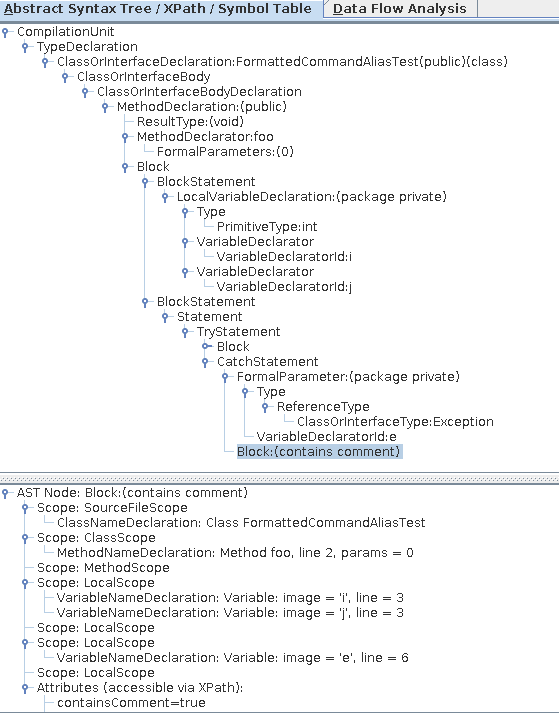
\includegraphics[height=30em]{pmd1.png}

\newpage
[Question 5 answer can start on previous page and continue here]
\newpage


%% Write an XPath expression that finds all siblings of the node with role "heading" and goes to their descendant with
%% property "autoid" and value "\_lvv\_5".

%% \begin{lstlisting}
%% <div role="heading" tabindex="-1"> ... </div>
%% <div id="_ariaId_29" ...>
%% <div class="_lvv_H _lvv_Q">
%% <span class="lvHighlightAllClass lvHighlightFromClass" autoid="_lvv_5">Jeffrey Zarnett</span>
%% </div>
%% </div>
%% \end{lstlisting}

\section{Input Generation [10 marks]}

Consider the following descriptions of room contents.
\begin{center}
\begin{minipage}{.3\textwidth}
\begin{lstlisting}
building dc
floor 2
room 2539
occupant plam
room 2523
occupant seadmin
occupant selounge
room 2531
occupant rbc
end-room
end-floor
room 2567
occupant upperyearlab
end-room
end-building
\end{lstlisting}
\end{minipage}\begin{minipage}{.3\textwidth} \begin{lstlisting}
building eit
floor 3
room 3146
occupant selounge
end-room
room 3141
occupant ecemeetings
end-room
end-floor
floor 1
occupant dinosaurs
end-floor
end-building
\end{lstlisting}
\end{minipage}
\end{center}
Write a grammar which can automatically generate such descriptions.
You can use terminals for OCCUPANT and BUILDING that you don't need to define.
Floors should be single digits and rooms should be four digits.
Describe how you would enforce the constraint that the room number
must start with the same digit as the floor.

\newpage
\end{document}
